
%%%% LOAD DOCUMENT CLASS

\documentclass[12pt,crest,nopardent,msfonts,fancychap,hyper,nomencl]{glaphdths}

%%%% SET THE PATH FOR DIAGRAMS.

\graphicspath{{chapter1/}{chapter2/}{chapter3/}{chapter4/}{chapter5/}}

%%%% TITLE DETAILS

%% Author
\author{Cristina Chueca Del Cerro, MRes, MA}

%% Title
\title{THIS IS MY \\
\LARGE THESIS TEMPLATE}

%% Qualification (Defaults to \textit{Doctor of Philosophy})
\qualification{\MakeUppercase{Submitted in fulfilment of the requirements for the Degree of \\
% \vspace{0.30cm}
Doctor of Philosophy}}

%% University (Defaults to \textsc{The University of Edinburgh})
 \university{\MakeUppercase{School of XXX \\
 \vspace{0.25cm}
 College of XXX}}

%% Year of submission
\date{\MakeUppercase{XX 202XX}}

%% add in bib file
\addbibresource{bib/bibliography.bib}

%%%% Wordcount -- check on Menu> Wordcount

%%%% START DOCUMENT

\setlength{\parskip}{1.5\baselineskip}

\begin{document}

%%%% FRONT MATTER
\let\cleardoublepage\clearpage

\makeprecontent{front/precntnt.tex}


\cleardoublepage%
%%%% START MAIN BODY TEXT

%% Call the glaphdths wrapper.
\startbody

\chapter{Introduction}

\blindtext
\chapter{CHAPTER NAME}

\section{Introduction}

Lorem ipsum dolor sit amet \parencite{Scherman21}, consectetuer adipiscing elit. Etiam lobortis facilisis sem. Nullam nec mi et neque pharetra sollicitudin. Praesent imperdiet mi nec ante. Donec ullamcorper, felis non sodales commodo, lectus velit ultrices augue, a dignissim nibhlectus placerat pede. Vivamus nunc nunc, molestie ut, ultricies vel, semper in, velit. Ut porttitor. Praesent in sapien. Lorem ipsum dolor sit amet, consectetuer adipiscing elit. Duis fringilla tristique neque \parencite{Moreno95,Turner92}. Sed interdum libero ut metus. Pellentesque placerat. Nam rutrum augue a leo. Morbi sed elit sit amet ante lobortis sollicitudin. Praesent blandit blandit mauris. Praesent lectus tellus, aliquet aliquam, luctus a, egestas a, turpis. Mauris lacinia lorem sit amet ipsum. Nunc quis urna dictum turpis accumsan semper Figure \ref{fig:NAME}. 

\begin{figure}[ht]
    \centering
    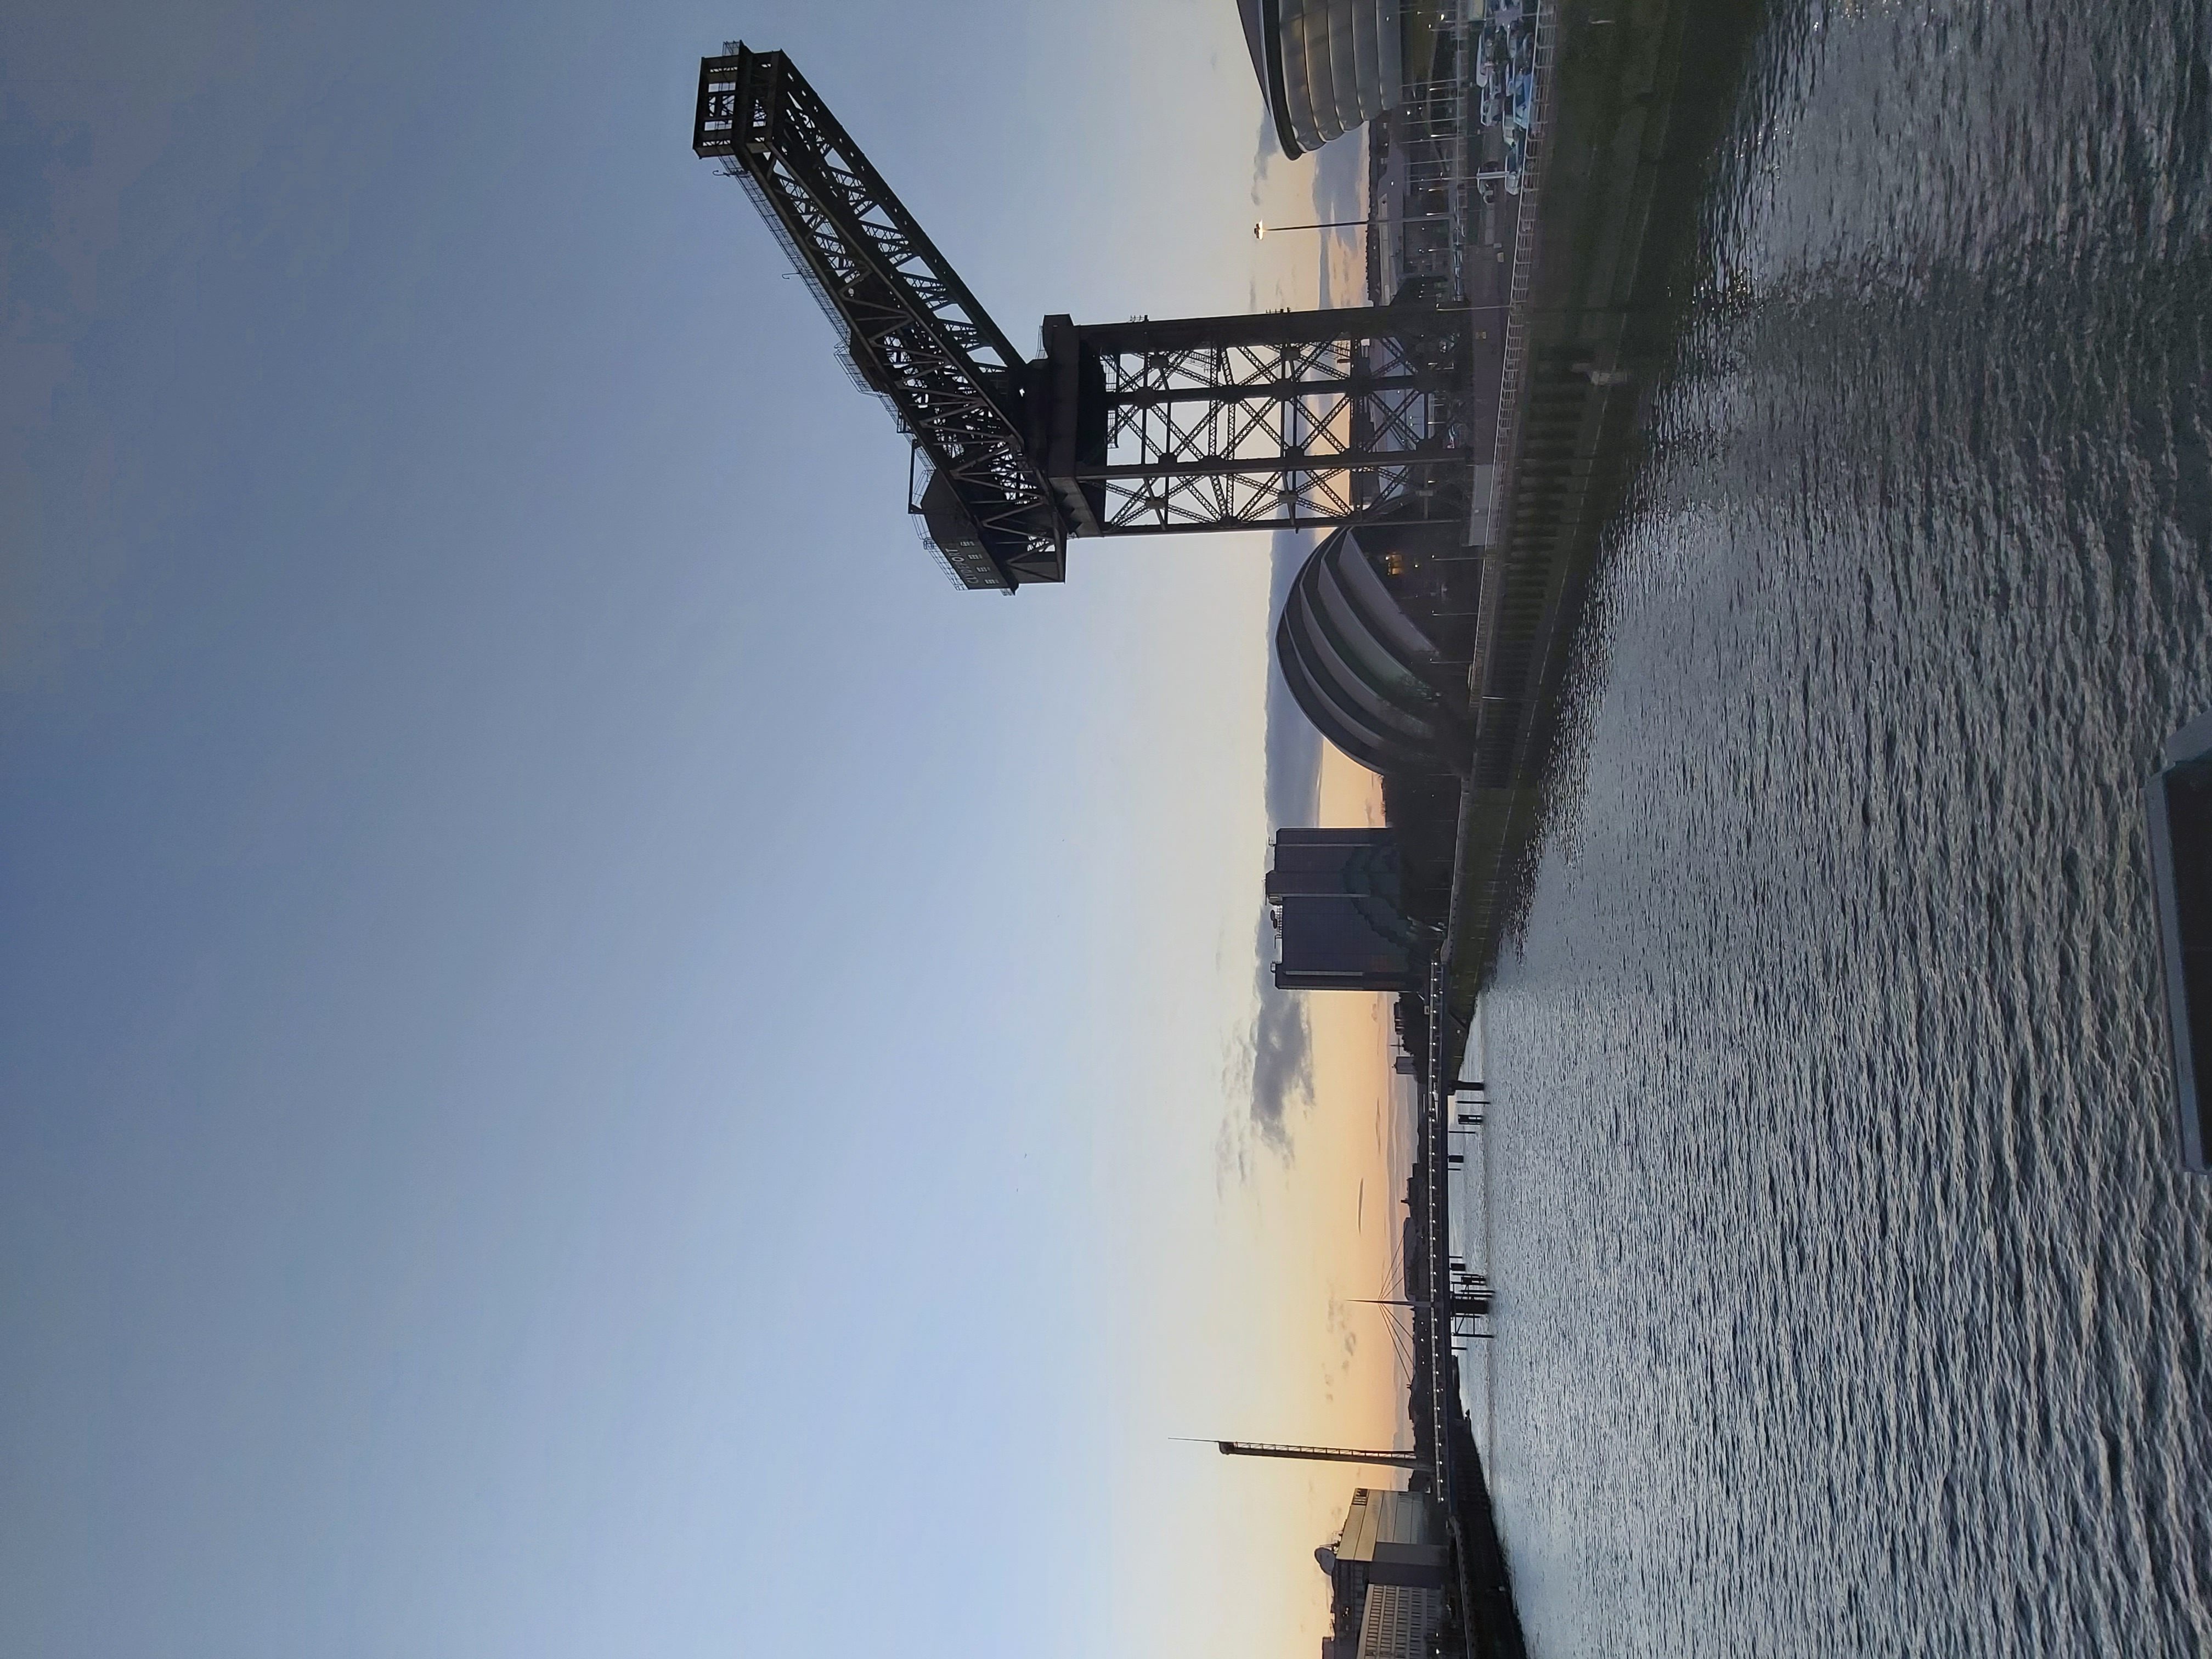
\includegraphics[width=\linewidth,angle =-90]{chapter2/Glasgow.jpg}
    \caption{Glasgow - River Clyde}
    \label{fig:NAME}
\end{figure}
 

\chapter{CHAPTER NAME}

  	
\subsubsection{Pseudocode}

Writing pseudocode:

\begin{algorithm}[H]
\SetAlgoLined
\label{alg:1}
\setstretch{1.35}
 Agent receives information from the weather app \;
 
 \eIf{Feeling good \textbf{and} have time}{
    Plan going out\;
   }{
    Remain home \;
  }
  \While{Condition C $\geq$ random number}{
  
  Do calculations \;
  Check the weather \;
  
  \eIf{d $\geq$ 0.5 and there is good weather } 
  {
   Go out without an umbrella
  }{
  Grab a jacket
  }
 }
 \KwResult{Going out for a walk}

  \caption{Walking decision}
\end{algorithm}


\chapter{CHAPTER NAME }

The results of the parameter sweeps were imported into \href{https://www.rstudio.com}{RStudio}, see Table \ref{tab:regression}.\\ 

\begin{table}[!ht]
\centering
\begin{adjustbox}{width=\textwidth}
\begin{tabular}{lcccc}
\toprule
\multicolumn{1}{c}{\multirow{2}[2]{*}{}} &  &  \textbf{Dependent Variables} &  & \\
\cline{2-5}\\
\multicolumn{1}{c}{\multirow{2}[2]{*}{\textbf{Independent Variables}}}  & Outcome 1 & Outcome 2 & Outcome 3 & Outcome 4  \\
\multicolumn{1}{c}{\multirow{2}{*}{ }} & Text  & Text  & Text  & Text \\
\toprule 
\textit{Variable 1} & \checkmark & \checkmark & \checkmark & \checkmark\\
\textit{Variable 2}& \checkmark & \checkmark & \checkmark & \checkmark \\
\textit{Variable 3}& \checkmark & \checkmark & \checkmark & \checkmark \\
\textit{Variable 4} &  & \checkmark & \checkmark & \checkmark\\
\textit{Variable 5} &  & & & \checkmark\\
\bottomrule
\end{tabular}
\end{adjustbox}
\caption[Regression Models Table]{Table caption}
\label{tab:regression}
\end{table}

The OLS models I propose is as follows:
\begin{align*}
\mathrm{Outcome}_{t} = X\beta_0 + X\beta_1 + X\beta_2 + X\beta_3 + \epsilon \\
    & + \mathrm{X}\beta_{2} X \times \mathrm{X}\beta_{3} + \epsilon \\
\end{align*}

Results of the regression model are presented in Table \ref{tab:OLS1}.\\  %this feels silly\\

\begin{table}[H] 
\centering 
\begin{adjustbox}{width=\textwidth}
\begin{tabular}{@{\extracolsep{5pt}}lD{.}{.}{-3} D{.}{.}{-3} }  
\\[-1.8ex]\hline 
\\[-1.8ex]\hline 
\hline \\[-1.8ex] 
 & \multicolumn{2}{c}{\textit{Dependent variable:}} \\ 
\cline{2-3} 
\\[-1.8ex] & \multicolumn{2}{c}{Measure} \\ 
\\[-1.8ex] & \multicolumn{1}{c}{Model (1)} & \multicolumn{1}{c}{Model (2)}\\ 
\hline \\[-1.8ex] 
  Constant & 0.215^{***} & 0.271^{***} \\ 
  & (0.009) & (0.010) \\ 
  & & \\ 
  Variable 1   & -0.067^{***} & -0.064^{***} \\ 
  & (0.003) & (0.003) \\ 
  & & \\ 
  Variable 2 & 0.063^{***} & -0.079^{***} \\ 
  & (0.003) & (0.014) \\ 
  & & \\ 
  Variable 3 & 0.085^{***} & 0.074^{***} \\ 
  & (0.009) & (0.008) \\ 
  & & \\ 
  Variable 4 & -0.158^{***} & -0.223^{***} \\ 
  & (0.010) & (0.011) \\ 
  & & \\ 
  Variable 3 : Variable 4 &  & 0.183^{***} \\ 
  &  & (0.017) \\ 
  & & \\ 
\hline \\[-1.8ex] 
Observations & \multicolumn{1}{c}{480} & \multicolumn{1}{c}{480} \\ 
Adjusted R$^{2}$ & \multicolumn{1}{c}{0.743} & \multicolumn{1}{c}{0.792} \\ 
Residual Std. Error & \multicolumn{1}{c}{0.032 (df = 475)} & \multicolumn{1}{c}{0.029 (df = 474)} \\ 
F Statistic & \multicolumn{1}{c}{346.682$^{***}$ (df = 4; 475)} & \multicolumn{1}{c}{366.066$^{***}$ (df = 5; 474)} \\ 
\hline 
\hline \\[-1.8ex] 
\textit{Note:}  & \multicolumn{1}{r}{$^{*}$p$<$0.1; $^{**}$p$<$0.05; $^{***}$p$<$0.01} \\ 
\end{tabular}
\end{adjustbox}
\caption{Table caption} 
\label{tab:OLS1}
\end{table} 

\chapter{Discussion}

\blindtext
\appendix
\chapter*{Appendices}% If \appendix doesn't insert a \chapter
\addcontentsline{toc}{chapter}{Appendices}% Print Appendix in ToC
\renewcommand{\thesection}{\Alph{section}}% Adjust section printing (from here onward)
\setcounter{table}{5}
\setcounter{figure}{5}


\section{Summary statistics Tables}
\label{appendix:1}

Table \ref{tab:NDSum} focuses on the parameters relevant for national identity dynamics whereas Table \ref{tab:NDSum1} focuses on the parameters relevant for the protest mobilisation dynamics.\\ 

\begin{table}[H]
\centering
\caption[NAME FOR TOC]{ GENERAL NAME FOR DISPLAY}
\label{tab:NDSum}
\begin{adjustbox}{width=\textwidth}
\begin{tabular}{|rcccccccc|}
  \hline
 & Variable 1 & Variable 2 & Variable 3 & Variable 4 & Variable 5 & Variable 6 & Variable 7 & Variable 8\\
  & 1.1 & 2.1 & 3.1 & 4.1 & 5.1 & 6.1 & 7.1 & 8.1\\
  \hline
1 & Condition X & Condition Z & 0.00 & 0.25 & 0.06 & 0.07 & 0.68 & 0.24 \\ 
  2 & Condition X & Condition Z & 0.10 & 0.25 & 0.06 & 0.07 & 0.81 & 0.25 \\ 
  3 & Condition X & Condition Z & 0.20 & 0.25 & 0.06 & 0.07 & 0.83 & 0.25 \\ 
  4 & Condition X & Condition Z & 0.30 & 0.25 & 0.06 & 0.07 & 0.84 & 0.25 \\ 
  5 & Condition X & Condition Z & 0.40 & 0.25 & 0.06 & 0.07 & 0.84 & 0.25 \\ 
  6 & Condition X & Condition Z & 0.50 & 0.25 & 0.06 & 0.06 & 0.85 & 0.25 \\ 
   \hline
  7 & Condition X & Condition A & 0.00 & 0.25 & 0.09 & 0.13 & 0.55 & 0.21 \\ 
  8 & Condition X & Condition A & 0.10 & 0.25 & 0.10 & 0.14 & 0.67 & 0.20 \\ 
  9 & Condition X & Condition A & 0.20 & 0.25 & 0.10 & 0.15 & 0.70 & 0.20 \\ 
  10 & Condition X & Condition A & 0.30 & 0.25 & 0.11 & 0.15 & 0.72 & 0.19 \\ 
  11 & Condition X & Condition A & 0.40 & 0.25 & 0.11 & 0.16 & 0.73 & 0.19 \\ 
  12 & Condition X & Condition A & 0.50 & 0.25 & 0.12 & 0.17 & 0.75 & 0.18 \\ 
   \hline
  13 & Condition Y & Condition Z & 0.00 & 0.25 & 0.08 & 0.10 & 0.76 & 0.22 \\ 
  14 & Condition Y & Condition Z & 0.10 & 0.25 & 0.08 & 0.10 & 0.89 & 0.22 \\ 
  15 & Condition Y & Condition Z & 0.20 & 0.25 & 0.08 & 0.09 & 0.91 & 0.23 \\ 
  16 & Condition Y & Condition Z & 0.30 & 0.25 & 0.07 & 0.09 & 0.92 & 0.23 \\ 
  17 & Condition Y & Condition Z & 0.40 & 0.25 & 0.07 & 0.09 & 0.93 & 0.23 \\ 
  18 & Condition Y & Condition Z & 0.50 & 0.25 & 0.07 & 0.09 & 0.93 & 0.23 \\ 
   \hline
  19 & Condition Y & Condition A & 0.00 & 0.25 & 0.17 & 0.26 & 0.65 & 0.12 \\ 
  20 & Condition Y & Condition A & 0.10 & 0.25 & 0.18 & 0.29 & 0.76 & 0.11 \\ 
  21 & Condition Y & Condition A & 0.20 & 0.25 & 0.19 & 0.31 & 0.78 & 0.11 \\ 
  22 & Condition Y & Condition A & 0.30 & 0.25 & 0.20 & 0.32 & 0.80 & 0.10 \\ 
  23 & Condition Y & Condition A & 0.40 & 0.25 & 0.21 & 0.33 & 0.81 & 0.10 \\ 
  24 & Condition Y & Condition A & 0.50 & 0.25 & 0.22 & 0.34 & 0.83 & 0.09 \\ 
   \hline
\end{tabular}
\end{adjustbox}
\end{table}


\newpage

%%% ALTERNATIVE TABLE FORMATTING

\begin{landscape}
\begin{longtable}{cc cc cc cc}
\caption[NAME FOR TOC ]{ GENERAL NAME FOR DISPLAY}
\label{tab:NDSum1}\\
\toprule
N
    &   \makecell[b]{Variable 1\\1.1 }
        &   \makecell[b]{Variable 2 \\ 2.1}  
           &   \makecell[b]{Variable 3 \\ 3.1 }
              &   \makecell[b]{Variable 4 \\4.1 }  
                 &   \makecell[b]{ Variable 5 \\ 5.1}
                   &   \makecell[b]{Variable 6\\ 6.1}
                     &   \makecell[b]{ Variable 7\\7.1 }  \\

    \midrule
\endfirsthead
    \midrule
    \multicolumn{8}{r}{\footnotesize\itshape Continue on the next page}
\endfoot
    \bottomrule
\endlastfoot

 1 & Condition Y & Condition Z & 0.00 &   0 & 0.10 & 0.05 & 0.00 \\ 
  2 & Condition Y & Condition Z & 0.00 &   0 & 0.20 & 0.05 & 0.00 \\ 
  3 & Condition Y & Condition Z & 0.00 &   0 & 0.30 & 0.06 & 0.00 \\ 
  4 & Condition Y & Condition Z & 0.00 &   0 & 0.40 & 0.06 & 0.00 \\ 
  5 & Condition Y & Condition Z & 0.00 &   0 & 0.50 & 0.06 & 0.00 \\ 
  6 & Condition Y & Condition Z & 0.00 &   5 & 0.10 & 0.11 & 0.00 \\ 
  7 & Condition Y & Condition Z & 0.00 &   5 & 0.20 & 0.11 & 0.00 \\ 
  8 & Condition Y & Condition Z & 0.00 &   5 & 0.30 & 0.11 & 0.00 \\ 
  9 & Condition Y & Condition Z & 0.00 &   5 & 0.40 & 0.12 & 0.00 \\ 
  10 & Condition Y & Condition Z & 0.00 &   5 & 0.50 & 0.11 & 0.00 \\ 
  11 & Condition Y & Condition Z & 0.00 &  10 & 0.10 & 0.16 & 0.00 \\ 
  12 & Condition Y & Condition Z & 0.00 &  10 & 0.20 & 0.16 & 0.00 \\ 
  13 & Condition Y & Condition Z & 0.00 &  10 & 0.30 & 0.17 & 0.00 \\ 
  14 & Condition Y & Condition Z & 0.00 &  10 & 0.40 & 0.17 & 0.00 \\ 
  15 & Condition Y & Condition Z & 0.00 &  10 & 0.50 & 0.18 & 0.00 \\ 
  16 & Condition Y & Condition Z & 0.00 &  15 & 0.10 & 0.22 & 0.00 \\ 
  17 & Condition Y & Condition Z & 0.00 &  15 & 0.20 & 0.23 & 0.00 \\ 
  18 & Condition Y & Condition Z & 0.00 &  15 & 0.30 & 0.24 & 0.00 \\ 
  19 & Condition Y & Condition Z & 0.00 &  15 & 0.40 & 0.24 & 0.00 \\ 
  20 & Condition Y & Condition Z & 0.00 &  15 & 0.50 & 0.24 & 0.00 \\ 
  21 & Condition Y & Condition Z & 0.00 &  20 & 0.10 & 0.27 & 0.00 \\ 
  22 & Condition Y & Condition Z & 0.00 &  20 & 0.20 & 0.29 & 0.01 \\ 
  23 & Condition Y & Condition Z & 0.00 &  20 & 0.30 & 0.29 & 0.01 \\ 
  24 & Condition Y & Condition Z & 0.00 &  20 & 0.40 & 0.31 & 0.01 \\ 
  25 & Condition Y & Condition Z & 0.00 &  20 & 0.50 & 0.31 & 0.01 \\ 
  26 & Condition Y & Condition Z & 0.00 &  25 & 0.10 & 0.34 & 0.02 \\ 
  27 & Condition Y & Condition Z & 0.00 &  25 & 0.20 & 0.36 & 0.03 \\ 
  28 & Condition Y & Condition Z & 0.00 &  25 & 0.30 & 0.36 & 0.04 \\ 
  29 & Condition Y & Condition Z & 0.00 &  25 & 0.40 & 0.38 & 0.07 \\ 
  30 & Condition Y & Condition Z & 0.00 &  25 & 0.50 & 0.38 & 0.07 \\ 
  31 & Condition Y & Condition Z & 0.00 &  30 & 0.10 & 0.40 & 0.12 \\ 
  32 & Condition Y & Condition Z & 0.00 &  30 & 0.20 & 0.42 & 0.16 \\ 
  33 & Condition Y & Condition Z & 0.00 &  30 & 0.30 & 0.42 & 0.13 \\ 
  34 & Condition Y & Condition Z & 0.00 &  30 & 0.40 & 0.45 & 0.26 \\ 
  35 & Condition Y & Condition Z & 0.00 &  30 & 0.50 & 0.46 & 0.31 \\ 
  36 & Condition Y & Condition Z & 0.10 &   0 & 0.10 & 0.05 & 0.00 \\ 
  37 & Condition Y & Condition Z & 0.10 &   0 & 0.20 & 0.06 & 0.00 \\ 
  38 & Condition Y & Condition Z & 0.10 &   0 & 0.30 & 0.05 & 0.00 \\ 
  39 & Condition Y & Condition Z & 0.10 &   0 & 0.40 & 0.05 & 0.00 \\ 
  40 & Condition Y & Condition Z & 0.10 &   0 & 0.50 & 0.05 & 0.00 \\ 
  41 & Condition Y & Condition Z & 0.10 &   5 & 0.10 & 0.10 & 0.00 \\ 
  42 & Condition Y & Condition Z & 0.10 &   5 & 0.20 & 0.11 & 0.00 \\ 
  43 & Condition Y & Condition Z & 0.10 &   5 & 0.30 & 0.11 & 0.00 \\ 
  44 & Condition Y & Condition Z & 0.10 &   5 & 0.40 & 0.12 & 0.00 \\ 
  45 & Condition Y & Condition Z & 0.10 &   5 & 0.50 & 0.11 & 0.00 \\ 
  46 & Condition Y & Condition Z & 0.10 &  10 & 0.10 & 0.16 & 0.00 \\ 
  47 & Condition Y & Condition Z & 0.10 &  10 & 0.20 & 0.17 & 0.00 \\ 
  48 & Condition Y & Condition Z & 0.10 &  10 & 0.30 & 0.17 & 0.00 \\ 
  49 & Condition Y & Condition Z & 0.10 &  10 & 0.40 & 0.17 & 0.00 \\ 
  50 & Condition Y & Condition Z & 0.10 &  10 & 0.50 & 0.17 & 0.00 \\ 
  51 & Condition Y & Condition Z & 0.10 &  15 & 0.10 & 0.22 & 0.00 \\ 
  52 & Condition Y & Condition Z & 0.10 &  15 & 0.20 & 0.23 & 0.00 \\ 
  53 & Condition Y & Condition Z & 0.10 &  15 & 0.30 & 0.23 & 0.00 \\ 
  54 & Condition Y & Condition Z & 0.10 &  15 & 0.40 & 0.24 & 0.00 \\ 
  55 & Condition Y & Condition Z & 0.10 &  15 & 0.50 & 0.24 & 0.00 \\ 
  56 & Condition Y & Condition Z & 0.10 &  20 & 0.10 & 0.27 & 0.00 \\ 
  57 & Condition Y & Condition Z & 0.10 &  20 & 0.20 & 0.29 & 0.01 \\ 
  58 & Condition Y & Condition Z & 0.10 &  20 & 0.30 & 0.29 & 0.01 \\ 
  59 & Condition Y & Condition Z & 0.10 &  20 & 0.40 & 0.30 & 0.01 \\ 
  60 & Condition Y & Condition Z & 0.10 &  20 & 0.50 & 0.31 & 0.01 \\ 
  61 & Condition Y & Condition Z & 0.10 &  25 & 0.10 & 0.34 & 0.02 \\ 
  62 & Condition Y & Condition Z & 0.10 &  25 & 0.20 & 0.35 & 0.02 \\ 
  63 & Condition Y & Condition Z & 0.10 &  25 & 0.30 & 0.37 & 0.05 \\ 
  64 & Condition Y & Condition Z & 0.10 &  25 & 0.40 & 0.36 & 0.04 \\ 
  65 & Condition Y & Condition Z & 0.10 &  25 & 0.50 & 0.38 & 0.06 \\ 
  66 & Condition Y & Condition Z & 0.10 &  30 & 0.10 & 0.41 & 0.14 \\ 
  67 & Condition Y & Condition Z & 0.10 &  30 & 0.20 & 0.42 & 0.13 \\ 
  68 & Condition Y & Condition Z & 0.10 &  30 & 0.30 & 0.44 & 0.21 \\ 
  69 & Condition Y & Condition Z & 0.10 &  30 & 0.40 & 0.44 & 0.19 \\ 
  70 & Condition Y & Condition Z & 0.10 &  30 & 0.50 & 0.44 & 0.21 \\ 
  71 & Condition Y & Condition Z & 0.20 &   0 & 0.10 & 0.05 & 0.00 \\ 
  72 & Condition Y & Condition Z & 0.20 &   0 & 0.20 & 0.05 & 0.00 \\ 
  73 & Condition Y & Condition Z & 0.20 &   0 & 0.30 & 0.05 & 0.00 \\ 
  74 & Condition Y & Condition Z & 0.20 &   0 & 0.40 & 0.05 & 0.00 \\ 
  75 & Condition Y & Condition Z & 0.20 &   0 & 0.50 & 0.05 & 0.00 \\ 
  76 & Condition Y & Condition Z & 0.20 &   5 & 0.10 & 0.10 & 0.00 \\ 
  77 & Condition Y & Condition Z & 0.20 &   5 & 0.20 & 0.11 & 0.00 \\ 
  78 & Condition Y & Condition Z & 0.20 &   5 & 0.30 & 0.12 & 0.00 \\ 
  79 & Condition Y & Condition Z & 0.20 &   5 & 0.40 & 0.11 & 0.00 \\ 
  80 & Condition Y & Condition Z & 0.20 &   5 & 0.50 & 0.12 & 0.00 \\ 
  81 & Condition Y & Condition Z & 0.20 &  10 & 0.10 & 0.16 & 0.00 \\ 
  82 & Condition Y & Condition Z & 0.20 &  10 & 0.20 & 0.17 & 0.00 \\ 
  83 & Condition Y & Condition Z & 0.20 &  10 & 0.30 & 0.17 & 0.00 \\ 
  84 & Condition Y & Condition Z & 0.20 &  10 & 0.40 & 0.17 & 0.00 \\ 
  85 & Condition Y & Condition Z & 0.20 &  10 & 0.50 & 0.18 & 0.00 \\ 
  86 & Condition Y & Condition Z & 0.20 &  15 & 0.10 & 0.22 & 0.00 \\ 
  87 & Condition Y & Condition Z & 0.20 &  15 & 0.20 & 0.23 & 0.00 \\ 
  88 & Condition Y & Condition Z & 0.20 &  15 & 0.30 & 0.23 & 0.00 \\ 
  89 & Condition Y & Condition Z & 0.20 &  15 & 0.40 & 0.23 & 0.00 \\ 
  90 & Condition Y & Condition Z & 0.20 &  15 & 0.50 & 0.24 & 0.00 \\ 
  91 & Condition Y & Condition Z & 0.20 &  20 & 0.10 & 0.29 & 0.01 \\ 
  92 & Condition Y & Condition Z & 0.20 &  20 & 0.20 & 0.29 & 0.01 \\ 
  93 & Condition Y & Condition Z & 0.20 &  20 & 0.30 & 0.29 & 0.01 \\ 
  94 & Condition Y & Condition Z & 0.20 &  20 & 0.40 & 0.30 & 0.01 \\ 
  95 & Condition Y & Condition Z & 0.20 &  20 & 0.50 & 0.31 & 0.01 \\ 
  96 & Condition Y & Condition Z & 0.20 &  25 & 0.10 & 0.34 & 0.02 \\ 
  97 & Condition Y & Condition Z & 0.20 &  25 & 0.20 & 0.35 & 0.03 \\ 
  98 & Condition Y & Condition Z & 0.20 &  25 & 0.30 & 0.36 & 0.04 \\ 
  99 & Condition Y & Condition Z & 0.20 &  25 & 0.40 & 0.37 & 0.05 \\ 
  100 & Condition Y & Condition Z & 0.20 &  25 & 0.50 & 0.37 & 0.04 \\ 
  101 & Condition Y & Condition Z & 0.20 &  30 & 0.10 & 0.41 & 0.12 \\ 
  102 & Condition Y & Condition Z & 0.20 &  30 & 0.20 & 0.41 & 0.12 \\ 
  103 & Condition Y & Condition Z & 0.20 &  30 & 0.30 & 0.42 & 0.15 \\ 
  104 & Condition Y & Condition Z & 0.20 &  30 & 0.40 & 0.45 & 0.26 \\ 
  105 & Condition Y & Condition Z & 0.20 &  30 & 0.50 & 0.45 & 0.25 \\ 
  106 & Condition Y & Condition Z & 0.30 &   0 & 0.10 & 0.05 & 0.00 \\ 
  107 & Condition Y & Condition Z & 0.30 &   0 & 0.20 & 0.05 & 0.00 \\ 
  108 & Condition Y & Condition Z & 0.30 &   0 & 0.30 & 0.05 & 0.00 \\ 
  109 & Condition Y & Condition Z & 0.30 &   0 & 0.40 & 0.05 & 0.00 \\ 
  110 & Condition Y & Condition Z & 0.30 &   0 & 0.50 & 0.06 & 0.00 \\ 
  111 & Condition Y & Condition Z & 0.30 &   5 & 0.10 & 0.10 & 0.00 \\ 
  112 & Condition Y & Condition Z & 0.30 &   5 & 0.20 & 0.11 & 0.00 \\ 
  113 & Condition Y & Condition Z & 0.30 &   5 & 0.30 & 0.11 & 0.00 \\ 
  114 & Condition Y & Condition Z & 0.30 &   5 & 0.40 & 0.12 & 0.00 \\ 
  115 & Condition Y & Condition Z & 0.30 &   5 & 0.50 & 0.12 & 0.00 \\ 
  116 & Condition Y & Condition Z & 0.30 &  10 & 0.10 & 0.17 & 0.00 \\ 
  117 & Condition Y & Condition Z & 0.30 &  10 & 0.20 & 0.17 & 0.00 \\ 
  118 & Condition Y & Condition Z & 0.30 &  10 & 0.30 & 0.17 & 0.00 \\ 
  119 & Condition Y & Condition Z & 0.30 &  10 & 0.40 & 0.17 & 0.00 \\ 
  120 & Condition Y & Condition Z & 0.30 &  10 & 0.50 & 0.17 & 0.00 \\ 
  121 & Condition Y & Condition Z & 0.30 &  15 & 0.10 & 0.22 & 0.00 \\ 
  122 & Condition Y & Condition Z & 0.30 &  15 & 0.20 & 0.22 & 0.00 \\ 
  123 & Condition Y & Condition Z & 0.30 &  15 & 0.30 & 0.22 & 0.00 \\ 
  124 & Condition Y & Condition Z & 0.30 &  15 & 0.40 & 0.24 & 0.00 \\ 
  125 & Condition Y & Condition Z & 0.30 &  15 & 0.50 & 0.24 & 0.00 \\ 
  126 & Condition Y & Condition Z & 0.30 &  20 & 0.10 & 0.28 & 0.00 \\ 
  127 & Condition Y & Condition Z & 0.30 &  20 & 0.20 & 0.28 & 0.00 \\ 
  128 & Condition Y & Condition Z & 0.30 &  20 & 0.30 & 0.30 & 0.01 \\ 
  129 & Condition Y & Condition Z & 0.30 &  20 & 0.40 & 0.30 & 0.01 \\ 
  130 & Condition Y & Condition Z & 0.30 &  20 & 0.50 & 0.32 & 0.01 \\ 
  131 & Condition Y & Condition Z & 0.30 &  25 & 0.10 & 0.35 & 0.03 \\ 
  132 & Condition Y & Condition Z & 0.30 &  25 & 0.20 & 0.35 & 0.03 \\ 
  133 & Condition Y & Condition Z & 0.30 &  25 & 0.30 & 0.37 & 0.05 \\ 
  134 & Condition Y & Condition Z & 0.30 &  25 & 0.40 & 0.37 & 0.06 \\ 
  135 & Condition Y & Condition Z & 0.30 &  25 & 0.50 & 0.39 & 0.08 \\ 
  136 & Condition Y & Condition Z & 0.30 &  30 & 0.10 & 0.41 & 0.13 \\ 
  137 & Condition Y & Condition Z & 0.30 &  30 & 0.20 & 0.43 & 0.21 \\ 
  138 & Condition Y & Condition Z & 0.30 &  30 & 0.30 & 0.44 & 0.22 \\ 
  139 & Condition Y & Condition Z & 0.30 &  30 & 0.40 & 0.43 & 0.17 \\ 
  140 & Condition Y & Condition Z & 0.30 &  30 & 0.50 & 0.47 & 0.31 \\ 
  141 & Condition Y & Condition Z & 0.40 &   0 & 0.10 & 0.05 & 0.00 \\ 
  142 & Condition Y & Condition Z & 0.40 &   0 & 0.20 & 0.05 & 0.00 \\ 
  143 & Condition Y & Condition Z & 0.40 &   0 & 0.30 & 0.05 & 0.00 \\ 
  144 & Condition Y & Condition Z & 0.40 &   0 & 0.40 & 0.05 & 0.00 \\ 
  145 & Condition Y & Condition Z & 0.40 &   0 & 0.50 & 0.06 & 0.00 \\ 
  146 & Condition Y & Condition Z & 0.40 &   5 & 0.10 & 0.11 & 0.00 \\ 
  147 & Condition Y & Condition Z & 0.40 &   5 & 0.20 & 0.11 & 0.00 \\ 
  148 & Condition Y & Condition Z & 0.40 &   5 & 0.30 & 0.11 & 0.00 \\ 
  149 & Condition Y & Condition Z & 0.40 &   5 & 0.40 & 0.12 & 0.00 \\ 
  150 & Condition Y & Condition Z & 0.40 &   5 & 0.50 & 0.12 & 0.00 \\ 
  151 & Condition Y & Condition Z & 0.40 &  10 & 0.10 & 0.16 & 0.00 \\ 
  152 & Condition Y & Condition Z & 0.40 &  10 & 0.20 & 0.17 & 0.00 \\ 
  153 & Condition Y & Condition Z & 0.40 &  10 & 0.30 & 0.17 & 0.00 \\ 
  154 & Condition Y & Condition Z & 0.40 &  10 & 0.40 & 0.17 & 0.00 \\ 
  155 & Condition Y & Condition Z & 0.40 &  10 & 0.50 & 0.18 & 0.00 \\ 
  156 & Condition Y & Condition Z & 0.40 &  15 & 0.10 & 0.22 & 0.00 \\ 
  157 & Condition Y & Condition Z & 0.40 &  15 & 0.20 & 0.23 & 0.00 \\ 
  158 & Condition Y & Condition Z & 0.40 &  15 & 0.30 & 0.24 & 0.00 \\ 
  159 & Condition Y & Condition Z & 0.40 &  15 & 0.40 & 0.24 & 0.00 \\ 
  160 & Condition Y & Condition Z & 0.40 &  15 & 0.50 & 0.24 & 0.00 \\ 
  161 & Condition Y & Condition Z & 0.40 &  20 & 0.10 & 0.28 & 0.00 \\ 
  162 & Condition Y & Condition Z & 0.40 &  20 & 0.20 & 0.29 & 0.00 \\ 
  163 & Condition Y & Condition Z & 0.40 &  20 & 0.30 & 0.30 & 0.01 \\ 
  164 & Condition Y & Condition Z & 0.40 &  20 & 0.40 & 0.30 & 0.01 \\ 
  165 & Condition Y & Condition Z & 0.40 &  20 & 0.50 & 0.30 & 0.01 \\ 
  166 & Condition Y & Condition Z & 0.40 &  25 & 0.10 & 0.33 & 0.02 \\ 
  167 & Condition Y & Condition Z & 0.40 &  25 & 0.20 & 0.36 & 0.04 \\ 
  168 & Condition Y & Condition Z & 0.40 &  25 & 0.30 & 0.36 & 0.03 \\ 
  169 & Condition Y & Condition Z & 0.40 &  25 & 0.40 & 0.37 & 0.04 \\ 
  170 & Condition Y & Condition Z & 0.40 &  25 & 0.50 & 0.37 & 0.05 \\ 
  171 & Condition Y & Condition Z & 0.40 &  30 & 0.10 & 0.41 & 0.14 \\ 
  172 & Condition Y & Condition Z & 0.40 &  30 & 0.20 & 0.41 & 0.13 \\ 
  173 & Condition Y & Condition Z & 0.40 &  30 & 0.30 & 0.43 & 0.19 \\ 
  174 & Condition Y & Condition Z & 0.40 &  30 & 0.40 & 0.45 & 0.26 \\ 
  175 & Condition Y & Condition Z & 0.40 &  30 & 0.50 & 0.45 & 0.25 \\ 
  176 & Condition Y & Condition Z & 0.50 &   0 & 0.10 & 0.05 & 0.00 \\ 
  177 & Condition Y & Condition Z & 0.50 &   0 & 0.20 & 0.05 & 0.00 \\ 
  178 & Condition Y & Condition Z & 0.50 &   0 & 0.30 & 0.05 & 0.00 \\ 
  179 & Condition Y & Condition Z & 0.50 &   0 & 0.40 & 0.05 & 0.00 \\ 
  180 & Condition Y & Condition Z & 0.50 &   0 & 0.50 & 0.06 & 0.00 \\ 
  181 & Condition Y & Condition Z & 0.50 &   5 & 0.10 & 0.10 & 0.00 \\ 
  182 & Condition Y & Condition Z & 0.50 &   5 & 0.20 & 0.11 & 0.00 \\ 
  183 & Condition Y & Condition Z & 0.50 &   5 & 0.30 & 0.11 & 0.00 \\ 
  184 & Condition Y & Condition Z & 0.50 &   5 & 0.40 & 0.11 & 0.00 \\ 
  185 & Condition Y & Condition Z & 0.50 &   5 & 0.50 & 0.12 & 0.00 \\ 
  186 & Condition Y & Condition Z & 0.50 &  10 & 0.10 & 0.15 & 0.00 \\ 
  187 & Condition Y & Condition Z & 0.50 &  10 & 0.20 & 0.17 & 0.00 \\ 
  188 & Condition Y & Condition Z & 0.50 &  10 & 0.30 & 0.17 & 0.00 \\ 
  189 & Condition Y & Condition Z & 0.50 &  10 & 0.40 & 0.17 & 0.00 \\ 
  190 & Condition Y & Condition Z & 0.50 &  10 & 0.50 & 0.17 & 0.00 \\ 
  191 & Condition Y & Condition Z & 0.50 &  15 & 0.10 & 0.21 & 0.00 \\ 
  192 & Condition Y & Condition Z & 0.50 &  15 & 0.20 & 0.23 & 0.00 \\ 
  193 & Condition Y & Condition Z & 0.50 &  15 & 0.30 & 0.23 & 0.00 \\ 
  194 & Condition Y & Condition Z & 0.50 &  15 & 0.40 & 0.24 & 0.00 \\ 
  195 & Condition Y & Condition Z & 0.50 &  15 & 0.50 & 0.23 & 0.00 \\ 
  196 & Condition Y & Condition Z & 0.50 &  20 & 0.10 & 0.27 & 0.00 \\ 
  197 & Condition Y & Condition Z & 0.50 &  20 & 0.20 & 0.28 & 0.00 \\ 
  198 & Condition Y & Condition Z & 0.50 &  20 & 0.30 & 0.29 & 0.00 \\ 
  199 & Condition Y & Condition Z & 0.50 &  20 & 0.40 & 0.30 & 0.01 \\ 
  200 & Condition Y & Condition Z & 0.50 &  20 & 0.50 & 0.32 & 0.01 \\ 
  201 & Condition Y & Condition Z & 0.50 &  25 & 0.10 & 0.34 & 0.02 \\ 
  202 & Condition Y & Condition Z & 0.50 &  25 & 0.20 & 0.36 & 0.03 \\ 
  203 & Condition Y & Condition Z & 0.50 &  25 & 0.30 & 0.36 & 0.04 \\ 
  204 & Condition Y & Condition Z & 0.50 &  25 & 0.40 & 0.36 & 0.03 \\ 
  205 & Condition Y & Condition Z & 0.50 &  25 & 0.50 & 0.39 & 0.07 \\ 
  206 & Condition Y & Condition Z & 0.50 &  30 & 0.10 & 0.41 & 0.15 \\ 
  207 & Condition Y & Condition Z & 0.50 &  30 & 0.20 & 0.43 & 0.17 \\ 
  208 & Condition Y & Condition Z & 0.50 &  30 & 0.30 & 0.43 & 0.17 \\ 
  209 & Condition Y & Condition Z & 0.50 &  30 & 0.40 & 0.45 & 0.25 \\ 
  210 & Condition Y & Condition Z & 0.50 &  30 & 0.50 & 0.55 & 0.48 \\ 
  \hline
  211 & Condition Y & Condition A & 0.00 &   0 & 0.10 & 0.05 & 0.00 \\ 
  212 & Condition Y & Condition A & 0.00 &   0 & 0.20 & 0.06 & 0.00 \\ 
  213 & Condition Y & Condition A & 0.00 &   0 & 0.30 & 0.05 & 0.00 \\ 
  214 & Condition Y & Condition A & 0.00 &   0 & 0.40 & 0.06 & 0.00 \\ 
  215 & Condition Y & Condition A & 0.00 &   0 & 0.50 & 0.06 & 0.00 \\ 
  216 & Condition Y & Condition A & 0.00 &   5 & 0.10 & 0.10 & 0.00 \\ 
  217 & Condition Y & Condition A & 0.00 &   5 & 0.20 & 0.11 & 0.00 \\ 
  218 & Condition Y & Condition A & 0.00 &   5 & 0.30 & 0.12 & 0.00 \\ 
  219 & Condition Y & Condition A & 0.00 &   5 & 0.40 & 0.11 & 0.00 \\ 
  220 & Condition Y & Condition A & 0.00 &   5 & 0.50 & 0.11 & 0.00 \\ 
  221 & Condition Y & Condition A & 0.00 &  10 & 0.10 & 0.16 & 0.00 \\ 
  222 & Condition Y & Condition A & 0.00 &  10 & 0.20 & 0.17 & 0.00 \\ 
  223 & Condition Y & Condition A & 0.00 &  10 & 0.30 & 0.17 & 0.00 \\ 
  224 & Condition Y & Condition A & 0.00 &  10 & 0.40 & 0.18 & 0.00 \\ 
  225 & Condition Y & Condition A & 0.00 &  10 & 0.50 & 0.17 & 0.00 \\ 
  226 & Condition Y & Condition A & 0.00 &  15 & 0.10 & 0.21 & 0.00 \\ 
  227 & Condition Y & Condition A & 0.00 &  15 & 0.20 & 0.23 & 0.00 \\ 
  228 & Condition Y & Condition A & 0.00 &  15 & 0.30 & 0.23 & 0.00 \\ 
  229 & Condition Y & Condition A & 0.00 &  15 & 0.40 & 0.24 & 0.00 \\ 
  230 & Condition Y & Condition A & 0.00 &  15 & 0.50 & 0.24 & 0.00 \\ 
  231 & Condition Y & Condition A & 0.00 &  20 & 0.10 & 0.28 & 0.01 \\ 
  232 & Condition Y & Condition A & 0.00 &  20 & 0.20 & 0.29 & 0.01 \\ 
  233 & Condition Y & Condition A & 0.00 &  20 & 0.30 & 0.30 & 0.01 \\ 
  234 & Condition Y & Condition A & 0.00 &  20 & 0.40 & 0.30 & 0.01 \\ 
  235 & Condition Y & Condition A & 0.00 &  20 & 0.50 & 0.31 & 0.01 \\ 
  236 & Condition Y & Condition A & 0.00 &  25 & 0.10 & 0.34 & 0.02 \\ 
  237 & Condition Y & Condition A & 0.00 &  25 & 0.20 & 0.35 & 0.03 \\ 
  238 & Condition Y & Condition A & 0.00 &  25 & 0.30 & 0.37 & 0.05 \\ 
  239 & Condition Y & Condition A & 0.00 &  25 & 0.40 & 0.37 & 0.04 \\ 
  240 & Condition Y & Condition A & 0.00 &  25 & 0.50 & 0.38 & 0.06 \\ 
  241 & Condition Y & Condition A & 0.00 &  30 & 0.10 & 0.41 & 0.12 \\ 
  242 & Condition Y & Condition A & 0.00 &  30 & 0.20 & 0.42 & 0.15 \\ 
  243 & Condition Y & Condition A & 0.00 &  30 & 0.30 & 0.45 & 0.25 \\ 
  244 & Condition Y & Condition A & 0.00 &  30 & 0.40 & 0.45 & 0.22 \\ 
  245 & Condition Y & Condition A & 0.00 &  30 & 0.50 & 0.47 & 0.33 \\ 
  246 & Condition Y & Condition A & 0.10 &   0 & 0.10 & 0.05 & 0.00 \\ 
  247 & Condition Y & Condition A & 0.10 &   0 & 0.20 & 0.05 & 0.00 \\ 
  248 & Condition Y & Condition A & 0.10 &   0 & 0.30 & 0.05 & 0.00 \\ 
  249 & Condition Y & Condition A & 0.10 &   0 & 0.40 & 0.05 & 0.00 \\ 
  250 & Condition Y & Condition A & 0.10 &   0 & 0.50 & 0.05 & 0.00 \\ 
  251 & Condition Y & Condition A & 0.10 &   5 & 0.10 & 0.11 & 0.00 \\ 
  252 & Condition Y & Condition A & 0.10 &   5 & 0.20 & 0.11 & 0.00 \\ 
  253 & Condition Y & Condition A & 0.10 &   5 & 0.30 & 0.11 & 0.00 \\ 
  254 & Condition Y & Condition A & 0.10 &   5 & 0.40 & 0.11 & 0.00 \\ 
  255 & Condition Y & Condition A & 0.10 &   5 & 0.50 & 0.11 & 0.00 \\ 
  256 & Condition Y & Condition A & 0.10 &  10 & 0.10 & 0.16 & 0.00 \\ 
  257 & Condition Y & Condition A & 0.10 &  10 & 0.20 & 0.17 & 0.00 \\ 
  258 & Condition Y & Condition A & 0.10 &  10 & 0.30 & 0.18 & 0.00 \\ 
  259 & Condition Y & Condition A & 0.10 &  10 & 0.40 & 0.18 & 0.00 \\ 
  260 & Condition Y & Condition A & 0.10 &  10 & 0.50 & 0.18 & 0.00 \\ 
  261 & Condition Y & Condition A & 0.10 &  15 & 0.10 & 0.22 & 0.00 \\ 
  262 & Condition Y & Condition A & 0.10 &  15 & 0.20 & 0.23 & 0.00 \\ 
  263 & Condition Y & Condition A & 0.10 &  15 & 0.30 & 0.23 & 0.00 \\ 
  264 & Condition Y & Condition A & 0.10 &  15 & 0.40 & 0.24 & 0.00 \\ 
  265 & Condition Y & Condition A & 0.10 &  15 & 0.50 & 0.24 & 0.00 \\ 
  266 & Condition Y & Condition A & 0.10 &  20 & 0.10 & 0.28 & 0.00 \\ 
  267 & Condition Y & Condition A & 0.10 &  20 & 0.20 & 0.29 & 0.01 \\ 
  268 & Condition Y & Condition A & 0.10 &  20 & 0.30 & 0.29 & 0.01 \\ 
  269 & Condition Y & Condition A & 0.10 &  20 & 0.40 & 0.29 & 0.01 \\ 
  270 & Condition Y & Condition A & 0.10 &  20 & 0.50 & 0.30 & 0.01 \\ 
  271 & Condition Y & Condition A & 0.10 &  25 & 0.10 & 0.34 & 0.02 \\ 
  272 & Condition Y & Condition A & 0.10 &  25 & 0.20 & 0.34 & 0.02 \\ 
  273 & Condition Y & Condition A & 0.10 &  25 & 0.30 & 0.36 & 0.03 \\ 
  274 & Condition Y & Condition A & 0.10 &  25 & 0.40 & 0.37 & 0.05 \\ 
  275 & Condition Y & Condition A & 0.10 &  25 & 0.50 & 0.38 & 0.05 \\ 
  276 & Condition Y & Condition A & 0.10 &  30 & 0.10 & 0.40 & 0.12 \\ 
  277 & Condition Y & Condition A & 0.10 &  30 & 0.20 & 0.41 & 0.13 \\ 
  278 & Condition Y & Condition A & 0.10 &  30 & 0.30 & 0.43 & 0.16 \\ 
  279 & Condition Y & Condition A & 0.10 &  30 & 0.40 & 0.44 & 0.21 \\ 
  280 & Condition Y & Condition A & 0.10 &  30 & 0.50 & 0.50 & 0.35 \\ 
  281 & Condition Y & Condition A & 0.20 &   0 & 0.10 & 0.05 & 0.00 \\ 
  282 & Condition Y & Condition A & 0.20 &   0 & 0.20 & 0.05 & 0.00 \\ 
  283 & Condition Y & Condition A & 0.20 &   0 & 0.30 & 0.06 & 0.00 \\ 
  284 & Condition Y & Condition A & 0.20 &   0 & 0.40 & 0.06 & 0.00 \\ 
  285 & Condition Y & Condition A & 0.20 &   0 & 0.50 & 0.06 & 0.00 \\ 
  286 & Condition Y & Condition A & 0.20 &   5 & 0.10 & 0.10 & 0.00 \\ 
  287 & Condition Y & Condition A & 0.20 &   5 & 0.20 & 0.11 & 0.00 \\ 
  288 & Condition Y & Condition A & 0.20 &   5 & 0.30 & 0.11 & 0.00 \\ 
  289 & Condition Y & Condition A & 0.20 &   5 & 0.40 & 0.12 & 0.00 \\ 
  290 & Condition Y & Condition A & 0.20 &   5 & 0.50 & 0.12 & 0.00 \\ 
  291 & Condition Y & Condition A & 0.20 &  10 & 0.10 & 0.16 & 0.00 \\ 
  292 & Condition Y & Condition A & 0.20 &  10 & 0.20 & 0.17 & 0.00 \\ 
  293 & Condition Y & Condition A & 0.20 &  10 & 0.30 & 0.17 & 0.00 \\ 
  294 & Condition Y & Condition A & 0.20 &  10 & 0.40 & 0.18 & 0.00 \\ 
  295 & Condition Y & Condition A & 0.20 &  10 & 0.50 & 0.18 & 0.00 \\ 
  296 & Condition Y & Condition A & 0.20 &  15 & 0.10 & 0.22 & 0.00 \\ 
  297 & Condition Y & Condition A & 0.20 &  15 & 0.20 & 0.23 & 0.00 \\ 
  298 & Condition Y & Condition A & 0.20 &  15 & 0.30 & 0.23 & 0.00 \\ 
  299 & Condition Y & Condition A & 0.20 &  15 & 0.40 & 0.24 & 0.00 \\ 
  300 & Condition Y & Condition A & 0.20 &  15 & 0.50 & 0.24 & 0.00 \\ 
  301 & Condition Y & Condition A & 0.20 &  20 & 0.10 & 0.28 & 0.00 \\ 
  302 & Condition Y & Condition A & 0.20 &  20 & 0.20 & 0.29 & 0.01 \\ 
  303 & Condition Y & Condition A & 0.20 &  20 & 0.30 & 0.29 & 0.01 \\ 
  304 & Condition Y & Condition A & 0.20 &  20 & 0.40 & 0.31 & 0.01 \\ 
  305 & Condition Y & Condition A & 0.20 &  20 & 0.50 & 0.31 & 0.01 \\ 
  306 & Condition Y & Condition A & 0.20 &  25 & 0.10 & 0.34 & 0.02 \\ 
  307 & Condition Y & Condition A & 0.20 &  25 & 0.20 & 0.36 & 0.03 \\ 
  308 & Condition Y & Condition A & 0.20 &  25 & 0.30 & 0.36 & 0.03 \\ 
  309 & Condition Y & Condition A & 0.20 &  25 & 0.40 & 0.37 & 0.05 \\ 
  310 & Condition Y & Condition A & 0.20 &  25 & 0.50 & 0.36 & 0.03 \\ 
  311 & Condition Y & Condition A & 0.20 &  30 & 0.10 & 0.41 & 0.12 \\ 
  312 & Condition Y & Condition A & 0.20 &  30 & 0.20 & 0.42 & 0.18 \\ 
  313 & Condition Y & Condition A & 0.20 &  30 & 0.30 & 0.44 & 0.20 \\ 
  314 & Condition Y & Condition A & 0.20 &  30 & 0.40 & 0.43 & 0.16 \\ 
  315 & Condition Y & Condition A & 0.20 &  30 & 0.50 & 0.47 & 0.34 \\ 
  316 & Condition Y & Condition A & 0.30 &   0 & 0.10 & 0.05 & 0.00 \\ 
  317 & Condition Y & Condition A & 0.30 &   0 & 0.20 & 0.06 & 0.00 \\ 
  318 & Condition Y & Condition A & 0.30 &   0 & 0.30 & 0.06 & 0.00 \\ 
  319 & Condition Y & Condition A & 0.30 &   0 & 0.40 & 0.06 & 0.00 \\ 
  320 & Condition Y & Condition A & 0.30 &   0 & 0.50 & 0.06 & 0.00 \\ 
  321 & Condition Y & Condition A & 0.30 &   5 & 0.10 & 0.10 & 0.00 \\ 
  322 & Condition Y & Condition A & 0.30 &   5 & 0.20 & 0.11 & 0.00 \\ 
  323 & Condition Y & Condition A & 0.30 &   5 & 0.30 & 0.11 & 0.00 \\ 
  324 & Condition Y & Condition A & 0.30 &   5 & 0.40 & 0.11 & 0.00 \\ 
  325 & Condition Y & Condition A & 0.30 &   5 & 0.50 & 0.12 & 0.00 \\ 
  326 & Condition Y & Condition A & 0.30 &  10 & 0.10 & 0.16 & 0.00 \\ 
  327 & Condition Y & Condition A & 0.30 &  10 & 0.20 & 0.17 & 0.00 \\ 
  328 & Condition Y & Condition A & 0.30 &  10 & 0.30 & 0.17 & 0.00 \\ 
  329 & Condition Y & Condition A & 0.30 &  10 & 0.40 & 0.18 & 0.00 \\ 
  330 & Condition Y & Condition A & 0.30 &  10 & 0.50 & 0.18 & 0.00 \\ 
  331 & Condition Y & Condition A & 0.30 &  15 & 0.10 & 0.22 & 0.00 \\ 
  332 & Condition Y & Condition A & 0.30 &  15 & 0.20 & 0.22 & 0.00 \\ 
  333 & Condition Y & Condition A & 0.30 &  15 & 0.30 & 0.23 & 0.00 \\ 
  334 & Condition Y & Condition A & 0.30 &  15 & 0.40 & 0.24 & 0.00 \\ 
  335 & Condition Y & Condition A & 0.30 &  15 & 0.50 & 0.24 & 0.00 \\ 
  336 & Condition Y & Condition A & 0.30 &  20 & 0.10 & 0.27 & 0.00 \\ 
  337 & Condition Y & Condition A & 0.30 &  20 & 0.20 & 0.29 & 0.00 \\ 
  338 & Condition Y & Condition A & 0.30 &  20 & 0.30 & 0.30 & 0.01 \\ 
  339 & Condition Y & Condition A & 0.30 &  20 & 0.40 & 0.30 & 0.01 \\ 
  340 & Condition Y & Condition A & 0.30 &  20 & 0.50 & 0.31 & 0.01 \\ 
  341 & Condition Y & Condition A & 0.30 &  25 & 0.10 & 0.34 & 0.02 \\ 
  342 & Condition Y & Condition A & 0.30 &  25 & 0.20 & 0.35 & 0.03 \\ 
  343 & Condition Y & Condition A & 0.30 &  25 & 0.30 & 0.37 & 0.05 \\ 
  344 & Condition Y & Condition A & 0.30 &  25 & 0.40 & 0.36 & 0.03 \\ 
  345 & Condition Y & Condition A & 0.30 &  25 & 0.50 & 0.36 & 0.03 \\ 
  346 & Condition Y & Condition A & 0.30 &  30 & 0.10 & 0.41 & 0.15 \\ 
  347 & Condition Y & Condition A & 0.30 &  30 & 0.20 & 0.42 & 0.15 \\ 
  348 & Condition Y & Condition A & 0.30 &  30 & 0.30 & 0.43 & 0.17 \\ 
  349 & Condition Y & Condition A & 0.30 &  30 & 0.40 & 0.44 & 0.24 \\ 
  350 & Condition Y & Condition A & 0.30 &  30 & 0.50 & 0.46 & 0.28 \\ 
  351 & Condition Y & Condition A & 0.40 &   0 & 0.10 & 0.05 & 0.00 \\ 
  352 & Condition Y & Condition A & 0.40 &   0 & 0.20 & 0.05 & 0.00 \\ 
  353 & Condition Y & Condition A & 0.40 &   0 & 0.30 & 0.05 & 0.00 \\ 
  354 & Condition Y & Condition A & 0.40 &   0 & 0.40 & 0.06 & 0.00 \\ 
  355 & Condition Y & Condition A & 0.40 &   0 & 0.50 & 0.06 & 0.00 \\ 
  356 & Condition Y & Condition A & 0.40 &   5 & 0.10 & 0.10 & 0.00 \\ 
  357 & Condition Y & Condition A & 0.40 &   5 & 0.20 & 0.11 & 0.00 \\ 
  358 & Condition Y & Condition A & 0.40 &   5 & 0.30 & 0.12 & 0.00 \\ 
  359 & Condition Y & Condition A & 0.40 &   5 & 0.40 & 0.11 & 0.00 \\ 
  360 & Condition Y & Condition A & 0.40 &   5 & 0.50 & 0.12 & 0.00 \\ 
  361 & Condition Y & Condition A & 0.40 &  10 & 0.10 & 0.16 & 0.00 \\ 
  362 & Condition Y & Condition A & 0.40 &  10 & 0.20 & 0.17 & 0.00 \\ 
  363 & Condition Y & Condition A & 0.40 &  10 & 0.30 & 0.17 & 0.00 \\ 
  364 & Condition Y & Condition A & 0.40 &  10 & 0.40 & 0.18 & 0.00 \\ 
  365 & Condition Y & Condition A & 0.40 &  10 & 0.50 & 0.18 & 0.00 \\ 
  366 & Condition Y & Condition A & 0.40 &  15 & 0.10 & 0.22 & 0.00 \\ 
  367 & Condition Y & Condition A & 0.40 &  15 & 0.20 & 0.23 & 0.00 \\ 
  368 & Condition Y & Condition A & 0.40 &  15 & 0.30 & 0.23 & 0.00 \\ 
  369 & Condition Y & Condition A & 0.40 &  15 & 0.40 & 0.24 & 0.00 \\ 
  370 & Condition Y & Condition A & 0.40 &  15 & 0.50 & 0.23 & 0.00 \\ 
  371 & Condition Y & Condition A & 0.40 &  20 & 0.10 & 0.28 & 0.00 \\ 
  372 & Condition Y & Condition A & 0.40 &  20 & 0.20 & 0.29 & 0.00 \\ 
  373 & Condition Y & Condition A & 0.40 &  20 & 0.30 & 0.30 & 0.01 \\ 
  374 & Condition Y & Condition A & 0.40 &  20 & 0.40 & 0.31 & 0.01 \\ 
  375 & Condition Y & Condition A & 0.40 &  20 & 0.50 & 0.31 & 0.01 \\ 
  376 & Condition Y & Condition A & 0.40 &  25 & 0.10 & 0.34 & 0.02 \\ 
  377 & Condition Y & Condition A & 0.40 &  25 & 0.20 & 0.36 & 0.04 \\ 
  378 & Condition Y & Condition A & 0.40 &  25 & 0.30 & 0.36 & 0.04 \\ 
  379 & Condition Y & Condition A & 0.40 &  25 & 0.40 & 0.37 & 0.05 \\ 
  380 & Condition Y & Condition A & 0.40 &  25 & 0.50 & 0.38 & 0.07 \\ 
  381 & Condition Y & Condition A & 0.40 &  30 & 0.10 & 0.40 & 0.12 \\ 
  382 & Condition Y & Condition A & 0.40 &  30 & 0.20 & 0.41 & 0.14 \\ 
  383 & Condition Y & Condition A & 0.40 &  30 & 0.30 & 0.44 & 0.20 \\ 
  384 & Condition Y & Condition A & 0.40 &  30 & 0.40 & 0.43 & 0.17 \\ 
  385 & Condition Y & Condition A & 0.40 &  30 & 0.50 & 0.44 & 0.21 \\ 
  386 & Condition Y & Condition A & 0.50 &   0 & 0.10 & 0.05 & 0.00 \\ 
  387 & Condition Y & Condition A & 0.50 &   0 & 0.20 & 0.05 & 0.00 \\ 
  388 & Condition Y & Condition A & 0.50 &   0 & 0.30 & 0.05 & 0.00 \\ 
  389 & Condition Y & Condition A & 0.50 &   0 & 0.40 & 0.06 & 0.00 \\ 
  390 & Condition Y & Condition A & 0.50 &   0 & 0.50 & 0.06 & 0.00 \\ 
  391 & Condition Y & Condition A & 0.50 &   5 & 0.10 & 0.10 & 0.00 \\ 
  392 & Condition Y & Condition A & 0.50 &   5 & 0.20 & 0.11 & 0.00 \\ 
  393 & Condition Y & Condition A & 0.50 &   5 & 0.30 & 0.11 & 0.00 \\ 
  394 & Condition Y & Condition A & 0.50 &   5 & 0.40 & 0.12 & 0.00 \\ 
  395 & Condition Y & Condition A & 0.50 &   5 & 0.50 & 0.12 & 0.00 \\ 
  396 & Condition Y & Condition A & 0.50 &  10 & 0.10 & 0.16 & 0.00 \\ 
  397 & Condition Y & Condition A & 0.50 &  10 & 0.20 & 0.17 & 0.00 \\ 
  398 & Condition Y & Condition A & 0.50 &  10 & 0.30 & 0.18 & 0.00 \\ 
  399 & Condition Y & Condition A & 0.50 &  10 & 0.40 & 0.18 & 0.00 \\ 
  400 & Condition Y & Condition A & 0.50 &  10 & 0.50 & 0.17 & 0.00 \\ 
  401 & Condition Y & Condition A & 0.50 &  15 & 0.10 & 0.23 & 0.00 \\ 
  402 & Condition Y & Condition A & 0.50 &  15 & 0.20 & 0.23 & 0.00 \\ 
  403 & Condition Y & Condition A & 0.50 &  15 & 0.30 & 0.23 & 0.00 \\ 
  404 & Condition Y & Condition A & 0.50 &  15 & 0.40 & 0.23 & 0.00 \\ 
  405 & Condition Y & Condition A & 0.50 &  15 & 0.50 & 0.24 & 0.00 \\ 
  406 & Condition Y & Condition A & 0.50 &  20 & 0.10 & 0.28 & 0.00 \\ 
  407 & Condition Y & Condition A & 0.50 &  20 & 0.20 & 0.28 & 0.00 \\ 
  408 & Condition Y & Condition A & 0.50 &  20 & 0.30 & 0.29 & 0.00 \\ 
  409 & Condition Y & Condition A & 0.50 &  20 & 0.40 & 0.31 & 0.01 \\ 
  410 & Condition Y & Condition A & 0.50 &  20 & 0.50 & 0.30 & 0.00 \\ 
  411 & Condition Y & Condition A & 0.50 &  25 & 0.10 & 0.34 & 0.02 \\ 
  412 & Condition Y & Condition A & 0.50 &  25 & 0.20 & 0.35 & 0.02 \\ 
  413 & Condition Y & Condition A & 0.50 &  25 & 0.30 & 0.35 & 0.02 \\ 
  414 & Condition Y & Condition A & 0.50 &  25 & 0.40 & 0.37 & 0.05 \\ 
  415 & Condition Y & Condition A & 0.50 &  25 & 0.50 & 0.38 & 0.05 \\ 
  416 & Condition Y & Condition A & 0.50 &  30 & 0.10 & 0.40 & 0.11 \\ 
  417 & Condition Y & Condition A & 0.50 &  30 & 0.20 & 0.42 & 0.15 \\ 
  418 & Condition Y & Condition A & 0.50 &  30 & 0.30 & 0.45 & 0.26 \\ 
  419 & Condition Y & Condition A & 0.50 &  30 & 0.40 & 0.44 & 0.20 \\ 
  420 & Condition Y & Condition A & 0.50 &  30 & 0.50 & 0.46 & 0.31 \\
 \hline
\end{longtable}
\end{landscape}

\newpage
 %merged appendices into one to avoid ToC clashes

\printbibliography


\end{document}
